%%% LaTeX Template: Article/Thesis/etc. with colored headings and special fonts
%%%
%%% Source: http://www.howtotex.com/

\documentclass[12pt]{article}


\usepackage{apuntes-estilo}
\usepackage{fancyhdr,lastpage}
\usepackage{color,colortbl}
\usepackage{float}
\usepackage{hyperref}
%\usepackage[dvips]{graphicx}

\def\maketitle{

% Titulo 
\makeatletter
{\color{bl} \centering \huge \sc \textbf{
Ofimática\\
 \vspace*{8pt} }\par}
 \makeatother


% Autor
 \makeatletter
 {\centering \small 
 	Departamento de Ingeniería de Computadoras \\
 	Facultad de Informática - Universidad Nacional del Comahue \\
 	\vspace{20pt} }
 \makeatother

}

% Custom headers and footers
\fancyhf{} % clear all header and footer fields
\fancypagestyle{plain}{\fancyhf{}}
  	\pagestyle{fancy}
 	\lhead{\footnotesize Ofimática - Departamento de Ingeniería de Computadoras}
 	\rhead{\footnotesize \thepage\ }	% "Page 1 of 2"

\def\ti#1#2{\texttt{#1} & #2 \\ }

\begin{document}

\thispagestyle{empty}
\maketitle
\setlength{\parindent}{0pt}


\section{Introducción}

En la mayoría de las oficinas, sean estas correspondientes a empresas, organismos gubernamentales o simplemente particulares, suelen utilizarse diversas herramientas informáticas con la finalidad de facilitar todas las tareas que se realizan.

Es por esta razón que quienes hacen este tipo de tareas deben estar correctamente capacitados en todas las aplicaciones que sean necesarias para un buen desempeño dentro de la organización. Por otro lado, es necesario que el informático a cargo de los sistemas, conozca las mejores aplicaciones para que luego pueda recomendar y adiestrar en el uso de las mismas. Además dado que todas las herramientas ofimáticas que se utilizan en las oficinas suelen actualizarse permanentemente, es importante que quienes estén encargados de utilizarlas también actualicen sus conocimientos.


\section{Qué es la Ofimática}

En primer lugar vamos a definir qué se entiende por Ofimática. Se llama Ofimática “al conjunto de técnicas, aplicaciones y herramientas informáticas que se utilizan en funciones de oficina para optimizar, automatizar, y mejorar tareas y procedimientos relacionados”\footnote{\url{http://es.wikipedia.org/wiki/Ofim\%E1tica}}.

Usando herramientas informáticas se puede crear, manipular, transmitir o almacenar la información necesaria en una oficina. Por otro lado, hoy en día la ofimática además requiere el uso de redes locales o de Internet, para que los usuarios puedan transmitir datos, correos electrónicos, etc.

\section{Herramientas Informáticas de Ofimática}

La ofimática surgió ante la necesidad de mecanizar las tareas que se desarrollaban en una oficina. Entonces aparecieron las máquinas de escribir y las fotocopiadoras. Aunque esto supuso un avance, la automatización se incrementó cuando aparecieron las computadoras personales. Entonces empezaron a surgir aplicaciones con un procesador de texto, agenda, calculadora, etc. 

Hoy en día, entre las herramientas informáticas que podemos encontrar hay:
\begin{itemize}
\item Procesadores de texto.
\item Planillas de cálculo.
\item Herramientas de presentación multimedia.
\item Base de datos.
\item Utilidades: agendas, calculadoras, etc.
\item Programas de correo electrónico, correo de voz, mensajeros.
\item Herramientas de reconocimiento y síntesis del habla.
\item Suite ofimática: paquete integrado de aplicaciones ofimática que se distribuyen en conjunto. 
\end{itemize}

Todas estas herramientas están disponibles para su uso en una PC y el producto de las mismas se guardan en unidades de almacenamiento, tales como discos duro, pendrive, etc. Sin embargo, como consecuencia del uso de Internet y el correo electrónico, han ido apareciendo nuevas soluciones ofimáticas basadas en cloud\footnote{\url{http://es.wikipedia.org/wiki/Computacion\_en\_la\_nube}}, las cuales ofrecen como ventajas, la accesibilidad a la documentación desde cualquier PC o dispositivo, facilitan la cooperación en la edición de la información y minimizan los riesgos de pérdida de datos por robo o ruptura del dispositivo. Entre estas soluciones podemos mencionar Google Drive, Zoho\footnote{\url{https://www.zoho.com/docs/}} y ThinkFree Cloud Office\footnote{\url{http://www.thinkfree.com/main.jsp}}.

\section{Suites Ofimática}

Una suite ofimática es un conjunto de aplicaciones utilizadas en oficinas y que permite contar con distintas funcionalidades. La mayoría, en general, incluye como mínimo un procesador de texto y una hoja de cálculo, pero algunas también incluyen una aplicación para realizar presentaciones,  un sistema de gestión de bases de datos, alguna herramienta básica para gráficos, e incluso aplicaciones para gestionar el correo electrónico y  la agenda.

Dentro de las suites propietarias se encuentra Microsoft Office. La primera versión fue lanzada en 1989 para incorporarla al primer Macintosh que desarrolló la empresa Apple. Luego, en 1990 apareció Microsoft Office para el sistema operativo Microsoft Windows. Esta primera versión contenía un procesador de textos (Microsoft Word), una hoja de cálculo (Microsoft Excel) y una aplicación para presentaciones (Microsoft PowerPoint). Además, se podía completar con la “versión profesional” que tenía una aplicación de bases de datos (Microsoft Access) y un gestor de información personal (Microsoft Schedule Plus) que más tarde se convertiría en lo que hoy conocemos como Microsoft Outlook.

Con el paso del tiempo, mientras Microsoft Office evolucionaba, comenzó el desarrollo de otra suite ofimática propietaria llamada StartOffice, perteneciente a la empresa StarDivision. Esta suite fue importante, ya que se convirtió en el punto de inicio de las herramientas libres de oficina. 

En 1999, la empresa Sun Microsystem adquirió a StarDivision y en el año 2000 liberó su código\footnote{\url{http://www.openoffice.org/press/sun\_release.html}} fuente bajo las licencias GNU GPL (General Public License), formando así la base para la suite de código abierto OpenOffice.org. Luego en 2010, Oracle compra Sun Microsystem y de ahí en adelante, como consecuencia de las decisiones que tomó la empresa con respecto al software, la mayoría del equipo de desarrollo de software decidió formar una organización sin fines de lucro llamada The Document Foundation y comenzó el desarrollo de LibreOffice a partir del código liberado de OpenOffice. Finalmente, Oracle donó la suite a Apache Software Foundation, una organización sin fines de lucro. De ahí que el nombre actual de la suite sea Apache OpenOffice\footnote{\url{https://www.openoffice.org/es/}}. 

Otras suites ofimáticas libres que surgieron fueron KOffice\footnote{\url{http://es.wikipedia.org/wiki/KOffice}} y GNOME Office. KOffice se lanzó por primera vez como parte de KDE2.0 para distribuciones Linux. A mediados de 2010, por desacuerdos entre los desarrolladores principales, la comunidad KOffice se dividió en dos comunidades separadas, KOffice y Calligra\footnote{\url{http://es.wikipedia.org/wiki/Calligra\_Suite}}. Actualmente se ha discontinuado el desarrollo de KOffice mientras que Calligra Suite está vigente.

Por otro lado Gnome Office es una suite desarrollada por el proyecto libre GNOME. Es una suite especial porque además incluye aplicaciones que han adoptado pero que no han sido desarrolladas por ellos, tal como Gimp.  

Otra suite que podemos mencionar es IBM Lotus Symphony\footnote{\url{http://es.wikipedia.org/wiki/IBM\_Lotus\_Symphony}}, cuyo desarrollo basado en OpenOffice tuvo varias mejoras aportadas por IBM. Pero en 2011 esta variante se reintegró en el código de OpenOffice, ya que IBM donó el código fuente de IBM Lotus Symphony al proyecto OpenOffice de la Fundación Apache. 

\subsection{Apache OpenOffice}

Apache OpenOffice es una suite de oficina de código abierto que ofrece herramientas para el procesamiento de palabras, hojas de cálculo, presentaciones, gráficos, bases de datos y más. La versión 4.1.1 está disponible bajo la Licencia Apache 2.0 \footnote{\url{http://www.apache.org/licenses/LICENSE-2.0.html}}, la cual permite descargar gratuitamente de Internet, copiar y redistribuir el software.   

Actualmente hay una comunidad trabajando en el desarrollo de OpenOffice, por lo cual podemos encontrar versiones actualizadas y mejoradas del mismo.

Por otro lado, existen versiones para varios idiomas y la versión de la que hablaremos (4.1.1) es compatible con los sistemas Windows (32 bits), GNU/Linux (32 y 64 bits) y Mac OS X. Esto representa una ventaja, ya que es posible editar los documentos en un entorno distinto al de creación del mismo.

En cuanto al formato predeterminado, la suite utiliza el OpenDocument (ODF) 1.2, un formato de archivo abierto para el almacenamiento de documentos ofimáticos, que además es un estándar a nivel internacional. Un archivo con este formato es un archivo comprimido en un contenedor ZIP, que contiene varios archivos y directorios. Los documentos ODF tienen las siguientes extensiones:
\begin{itemize}
\item *.odt (documentos de procesador de textos)
\item *.ods (documentos de libros de hojas de cálculo)
\item *.odp (documentos de presentaciones)
\item *.odb (documentos de base de datos)
\item *.odg (documento de la aplicación de dibujo vectorial)
\end{itemize}

Cabe destacar así mismo, que a la fecha de edición de este documento, la especificación de la versión 1.2 de OpenDocument ha sido presentada al Comité Conjunto ISO/IEC JTC para su aprobación como Norma Internacional\footnote{\url{http://www.iso.org/iso/home/store/catalogue\_tc/catalogue\_detail.htm?csnumber=66363}}

Sin embargo, además de este formato, OpenOffice permite trabajar con otros formatos\footnote{\url{https://wiki.openoffice.org/wiki/Documentation/OOo3\_User\_Guides/Getting\_Started/File\_formats}}. Tiene un gran porcentaje de compatibilidad con Microsoft Office, por lo que los documentos de texto, las hojas de cálculo y las presentaciones de MS Office se pueden abrir, editar y guardar de manera satisfactoria con OpenOffice. La suite también permite guardar documentos en formatos tales como RTF, TXT, Microsoft Office XML y OpenOffice.org XML. Adicionalmente puede exportar documentos directamente al formato PDF y exportar presentaciones al formato Adobe Flash (SWF). OpenOffice.org también cuenta con la capacidad de importar documentos en modo de «sólo lectura» en los formatos Unified Office Format, Data Interchange Format y los formatos propios de Microsoft Works, WordPerfect, Lotus 1-2-3, entre otros.

La suite consta de las siguientes aplicaciones\footnote{\url{https://www.openoffice.org/es/producto/index.html}}:
\begin{itemize}
\item Writer: un procesador de textos.
\item Calc: hoja de cálculo.
\item Draw: editor de dibujos y gráficos.
\item Impress: editor de presentaciones multimedia.
\item Base: permite la manipulación completa de base de datos
\item Math: editor de fórmulas matemáticas.
\end{itemize}

\subsubsection{Interfaz gráfica}

Todas las aplicaciones que componen la suite, comparten muchas características en su interfaz gráfica\footnote{\url{https://wiki.openoffice.org/wiki/ES/Manuales/GuiaAOO/UI}}. Veremos alguna de ellas, sin entrar en demasiado detalle. Entre los elementos básicos podemos encontrar los siguientes:

\begin{itemize}
\item \underline{Menú principal}: todas las aplicaciones tienen una estructura de menú principal semejante. En este menú se encuentran todas las funciones principales del programa, tales como crear un nuevo archivo, imprimir, dar formato al documento, la configuración del programa, etc.

\begin{figure}[H]
\centering
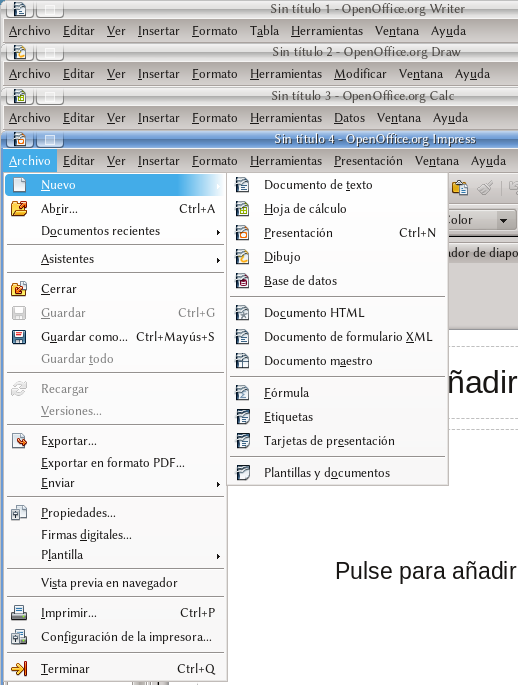
\includegraphics[width=0.8\textwidth]{menuAppsOO.png}
\renewcommand{\figurename}{Fig.}
\caption{Menú principal en aplicaciones de Apache OpenOffice}
\label{contexto:figura}
\end{figure}

\item \underline{Menú contextual}: realizando un clic derecho sobre un elemento del documento que se está revisando o sobre un elemento de la interfaz de usuario del programa, se presentará un menú con acciones relativas al elemento seleccionado. Por ejemplo, con un clic derecho sobre una palabra mal escrita se ofrecerán las opciones del corrector ortográfico, mientras que un clic derecho sobre una barra de herramientas permitirá acceder a las opciones de personalización de la misma.

\item \underline{Barras de herramientas}: una barra de herramientas es un elemento gráfico que contiene varios iconos los cuales permiten activar rápidamente distintas funciones del programa. Algunos de estos iconos ofrecen menús desplegables, otros muestran texto mientras que otros ofrecen funciones directas, como salvar el documento actual, etc.

\begin{figure}[h]
\centering
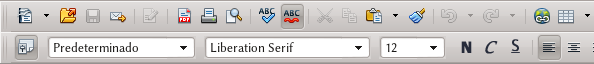
\includegraphics[width=0.8\textwidth]{barraHerramientaOO.png}
\renewcommand{\figurename}{Fig.}
\caption{Ejemplo Barra de herramientas en Apache OpenOffice Writer}
\label{contexto:figura}
\end{figure}

La lista de todas las barras de herramientas disponibles, se encuentra en el menú Ver $\rightarrow $ Barras de Herramientas. En este menú es posible activar barras que no son visibles como así también desactivar barras presentes en la interfaz.

Existen dos tipos de barras de herramientas: las «normales» que una vez activadas siempre se muestran y las «contextuales» que solo se muestran cuando se selecciona un objeto sobre el cual las herramientas de esa barra aplican. Ejemplo de barras contextuales son las de numeración y viñetas y la de edición de tablas en Writer, la barra de las propiedades de una imagen, la de las propiedades de un objeto gráfico (líneas, cuadros...), etc.

\item \underline{Barra de estado}: en la parte inferior de la ventana de la aplicación, se puede encontrar información sobre el documento. Por ejemplo, en Writer es posible ver, de izquierda a derecha: el número de página actual, el estilo de página, el idioma del texto en el que se encuentra el cursor, la modalidad del cursor, el modo de selección, mientras que a la derecha de la barra se encuentra la herramienta para controlar la escala del documento (si se ve al 100 \% o más, si se muestran dos páginas simultáneamente o solo una...)

\item \underline{Barra lateral}: a partir de Apache OpenOffice 4.0 se introdujo la Barra lateral como un nuevo elemento en la interfaz gráfica que facilita el acceso a las distintas herramientas ofrecidas por cada componente. En la siguiente captura, se la observa a la derecha:

\begin{figure}[H]
\centering
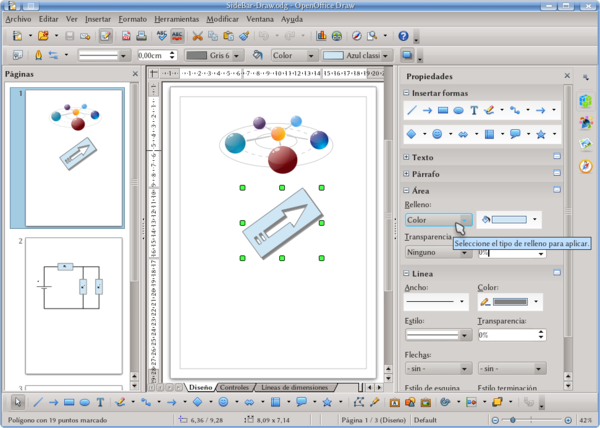
\includegraphics[width=0.8\textwidth]{barraLateralDrawOO.png}
\renewcommand{\figurename}{Fig.}
\caption{Ejemplo Barra lateral en Apache OpenOffice Writer}
\label{contexto:figura}
\end{figure}

\end{itemize}

\subsubsection{Instalación}

Tal como se indicara antes, OpenOffice es multiplataforma, por lo cual puede instalarse en sistemas Windows, GNU/Linux y Mac. En la página oficial, podemos encontrar la especificación completa de los requerimientos para realizar la instalación\footnote{\url{http://www.openoffice.org/dev\_docs/source/sys\_reqs\_aoo41.html}}. 

En lo que respecta a Windows, se requiere lo siguiente:
\begin{itemize}
\item Windows XP, Windows 2003, Windows Vista, Windows 7, Windows 8, Windows 8.1
\item 256 MB de RAM (se recomienda 512 MB RAM)
\item al menos 650 MB de espacio libre en disco para realizar una instalación vía download. Finalizada la instalación, se eliminan los archivos temporales de instalación y OpenOffice usará aproximadamente 440 MB de espacio en disco.
\item una resolución de pantalla de 1024 x 768 o superior con al menos 256 colores.
\end{itemize}

En lo que respecta a GNU/Linux, se requiere:
\begin{itemize}
\item Linux kernel versión 2.6 o superior, glibc2 versión 2.5 o superior
\item 256 MB de RAM (se recomienda 512 MB RAM)
\item 400 MB de espacio libre en disco
\item X-Server con una resolución de 1024 x 768 o superior con al menos 256 colores
\end{itemize}

Para realizar la instalación de OpenOffice es necesario tener instalado Java. 

\subsubsection{Configuración}

Hay varias cuestiones que pueden configurarse en OpenOffice, pero aquí solo vamos a mencionar una de ellas. Muchas veces notamos que el inicio de OpenOffice es un tanto lento. Esto puede mejorarse habilitando la carga de OpenOffice al inicio de sesión, pero esto implica que la aplicación va a utilizar memoria incluso cuando no sea utilizada. Por otro lado, esta opción no está disponible en todos los sistemas operativos.

También es posible modificar la cantidad de memoria que OpenOffice va a utilizar. Pero hay que tener en cuenta que hacer este cambio implica que va a quedar una menor cantidad de memoria disponible para otras aplicaciones. 

Para realizar esta configuración, nos dirigimos al menú Herramientas $ \rightarrow $ Opciones. Una vez allí seleccionamos en el árbol de opciones de la izquierda la opción OpenOffice, luego Memoria y veremos la siguiente ventana:

\begin{figure}[H]
\centering
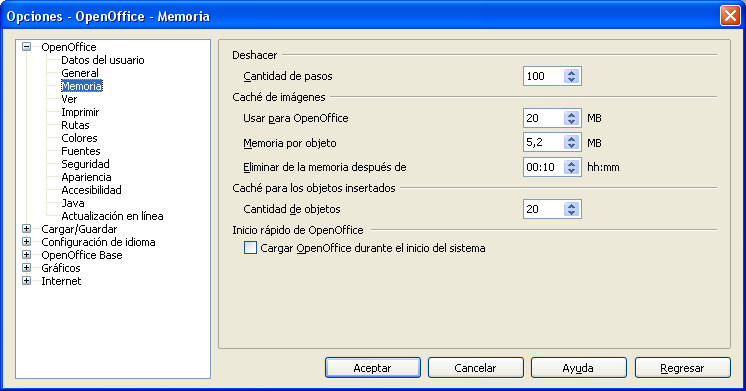
\includegraphics[width=1\textwidth]{configuracion_memoria_OO.png}
\renewcommand{\figurename}{Fig.}
\caption{Ventana configuración de memoria en OpenOffice}
\label{contexto:figura}
\end{figure}


\subsubsection{Uso de extensiones y plantillas para agregar funcionalidad}

Apache OpenOffice permite que el entorno de trabajo y ejecución sea ampliado, por medio de extensiones y plantillas.

Una extensión es una herramienta de terceros que agrega cierta función a la aplicación. En el caso de OpenOffice esto puede hacerse a través de add-ons y complementos, que utilizan la tecnología UNO (Universal Network Objects, objetos de red universales). Por ejemplo, en OpenOffice una extensión muy utilizada es el Diccionario de corrección ortográfica. Aunque se pueden encontrar extensiones en diferentes lugares, el repositorio oficial de extensiones para OpenOffice es \url{http://extensions.openoffice.org/}. 

Por otro lado, una plantilla es un documento diseñados para un uso específico y que puede utilizarse para crear otros documentos. Por ejemplo, un modelo de Curriculum Vitae. El repositorio oficial de plantillas para OpenOffice es \url{http://templates.openoffice.org/es}. También se pueden crear plantillas personales específicas para cualquier clase de documento (texto, hojas de cálculo, dibujo o presentación). Por ejemplo, se puede crear una plantilla para redactar las notas de una organización, que contenga el logotipo de la empresa en el encabezado. Todos los documentos nuevos creados a partir de esta plantilla, llevarán el logotipo de la empresa en el encabezado.

En cuanto a las extensiones o plantillas que incorporemos a OpenOffice, es necesario que prestemos atención al tipo de licencia bajo la cual se utiliza.

\subsubsection{Apache OpenOffice Portable}

La suite Apache OpenOffice también cuenta con una versión portable para Windows. Obviamente esto es particularmente útil cuando debemos acceder a nuestros documentos en un sistema en el que no está instalado el OpenOffice. Además utilizándolo de esta manera, uno puede continuar trabajando con las personalizaciones, extensiones, plantillas propias, etc, que uno configure en esta aplicación.

\subsection{LibreOffice}

Tal como se mencionara anteriormente, LibreOffice es una suite libre y gratuita, derivada de OpenOffice.org. Esta suite contiene un procesador de texto (Writer), presentaciones en diapositivas (Impress), una planilla de cálculo (Calc), un gestor de base de datos (Base), un programa de diseño de gráficos vectoriales (Draw) y un editor de fórmulas matemáticas (Math). Al igual que OpenOffice es multiplataforma, por lo cual puede usarse en sistemas Windows, GNU/Linux y Mac OS X. La versión actual a la fecha de edición de este documento es la 4.3 y de ella hablaremos.

Esta suite ha recibido el apoyo de la Free Software Foundation (FSF) por sobre OpenOffice, porque se distribuye con una licencia GPL totalmente libre. Aunque la FSF reconoce a OpenOffice como una parte importante dentro del ecosistema del software libre, el problema radica fundamentalmente en que se distribuye bajo los términos de la Licencia Apache\footnote{\url{http://es.wikipedia.org/wiki/Apache\_License}}. Esta licencia de software libre es sin copyleft, con lo cual alguien podría redistribuirlo bajo una licencia de software no libre. Por ello, la FSF presenta a LibreOffice como una alternativa que permite a los usuarios trabajar con una suite ofimática, protegiendo sus libertades.   

Por otro lado, esta suite es la que viene por defecto en la mayoría de las distribuciones de Linux, como Ubuntu o Debian, por ejemplo.

En cuanto al formato de archivo predeterminado, LibreOffice trabaja con el formato Open Document 1.2, pero también es compatible con otros formatos de documento utilizados por Microsoft Word, Excel, PowerPoint y Publisher. 

Además, LibreOffice ha incorporado importantes mejoras gráficas en el soporte del formato Open XML, mejorando la compatibilidad con las aplicaciones de la suite Microsoft Office. Así mismo, ahora soporta hojas de cálculo de Microsoft Works y bases de datos y una gran cantidad de formatos de archivos heredados de la plataforma Mac como ClarisWorks, ClarisResolve, MacWorks SuperPaint. 

En cuanto a todas las características que posee LibreOffice comparado con MS Office, podemos encontrar una especificación en \url{https://wiki.documentfoundation.org/Feature_Comparison:_LibreOffice_-_Microsoft_Office}

\subsubsection{Interfaz gráfica}

Al igual que en la suite Apache OpenOffice, todas las aplicaciones que componen LibreOffice tienen muchas características en común, tal como se puede observar en la siguiente imagen:

\begin{figure}[H]
\centering
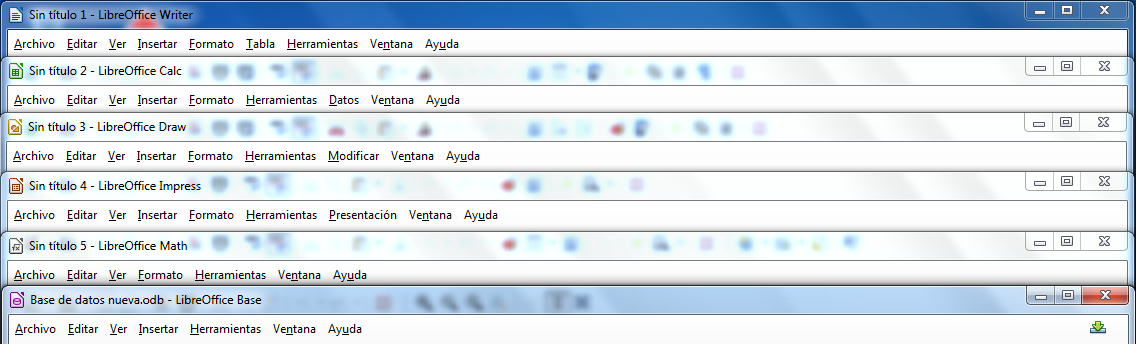
\includegraphics[width=1\textwidth]{menuAppsLO.png}
\renewcommand{\figurename}{Fig.}
\caption{Menú principal en aplicaciones de LibreOffice}
\label{contexto:figura}
\end{figure}

Así mismo, las características de cualquier interfaz gráfica como menú contextual, barra de herramientas, barra de estado, etc, las podemos encontrar en esta suite.

\begin{figure}[h]
\centering
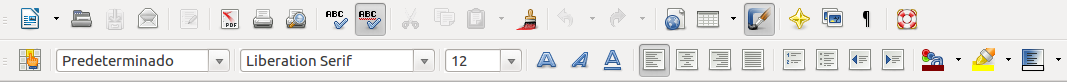
\includegraphics[width=0.9\textwidth]{barraHerramientaLO.png}
\renewcommand{\figurename}{Fig.}
\caption{Ejemplo Barra de herramientas en LibreOffice Writer}
\label{contexto:figura}
\end{figure}
 
\subsubsection{Instalación}

LibreOffice es una suite multiplataforma, por lo cual puede usarse en sistemas Windows, GNU/Linux y Mac. La página oficial en la que se encuentra la especificación de los requerimientos de instalación es \url{http://www.libreoffice.org/get-help/system-requirements/}.

En lo que respecta a Windows, los requisitos son los siguientes:
\begin{itemize}
\item Microsoft Windows XP, Vista, Windows 7, or Windows 8.
\item PC compatible con Pentium (Pentium III, Athlon o un sistema más reciente).
\item 256 MB de RAM (se recomienda 512 MB RAM).
\item 1.5 GB de espacio libre en disco.
\item Resolución de pantalla de 1024x768 (se recomienda una resolución superior), con al menos 256 colores.
\item Se necesitan derechos de Administrador para poder realizar el proceso de instalación.
\end{itemize}

En lo que respecta a sistemas GNU/Linux, los requisitos son los siguientes:
\begin{itemize}
\item Kernel de Linux versión 2.6.18 o superior.
\item glibc2 versión 2.5 o superior.
\item gtk versión 2.10.4 o superior.
\item PC compatible con Pentium (Pentium III, Athlon o sistemas más recientes);
\item 256 MB de RAM (se recomienda 512 MB RAM).
\item 1,55Gb de espacio libre en disco.
\item X Server con una resolución de 1024x768 (se recomienda mayor resolución), con al menos 256 colores;
\item Gnome 2.16 o superior, y paquetes gail 1.8.6 y spi-1.7 (necesarios para las herramientas de tecnología de asistencia [TA]), u otra interfaz gráfica de usuario compatible (por ejemplo, KDE).
\end{itemize}
Por supuesto, como regla general se recomienda instalar LibreOffice usando los métodos de instalación recomendados para la distribución de Linux que uno utilice. 

Tanto para la versión disponible para Windows como para GNU/Linux, ciertas características del software requieren la instalación de Java.

\subsubsection{Configuración}

LibreOffice también permite configurar varios componentes. De nuevo, solo nos vamos a enfocar en la configuraciones que nos permiten mejorar el rendimiento de la aplicación.

Una de las opciones es la relacionada con la gestión del uso de la memoria. LibreOffice permite modificar los parámetros relacionados con el consumo de memoria. Esta función resulta muy útil en equipos antiguos y con poca memoria RAM. Para configurar esto, nos dirigimos al menú Herramientas $\rightarrow $ Opciones. Luego en el árbol de la izquierda seleccionamos LibreOffice y a continuación Memoria. Desde ahí podemos gestionar el uso de la memoria en LibreOffice. La ventana que observamos es similar a la que muestra OpenOffice:

\begin{figure}[H]
\centering
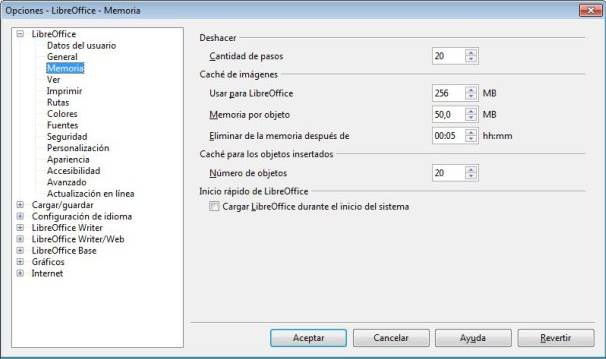
\includegraphics[width=1\textwidth]{configuracion_memoria_LO.png}
\renewcommand{\figurename}{Fig.}
\caption{Ventana configuración de memoria en LibreOffice}
\label{contexto:figura}
\end{figure}

Por otro lado, en el caso en que LibreOffice sea utilizado frecuentemente en un sistema Windows, es recomendable activar la carga de LibreOffice durante el inicio del sistema. Si, por el contrario, se usa solo ocasionalmente, es mejor desactivar esta opción, con lo que eliminamos un servicio en el arranque del sistema, acelerando su carga.

Otra opción está relacionada con el uso de Java. Aunque el uso del entorno viene activado por defecto en LibreOffice, la aplicación no lo necesita en todo momento para poder ejecutarse y esto consume recursos. Si se deshabilita Java se consigue que LibreOffice se ejecute mucho más rápido. La consecuencia negativa de hacer esto es que no se podrá utilizar los asistentes ni las macros, pero esto es usado por usuarios avanzados. También es posible que el módulo de trabajo Libre Office Base no se ejecute correctamente.

\subsubsection{Uso de extensiones y plantillas}

LibreOffice permite agregar funcionalidad a través de Extensiones. Muchas de estas son instaladas con la aplicación y otras pueden obtenerse desde el repositorio oficial \url {http://extensions.libreoffice.org/extension-center}. Todas las extensiones que pueden obtenerse desde allí están bajo  licencias de software libre.

También es posible agregar plantillas desde el repositorio oficial \url{http://templates.libreoffice.org/template-center}

\subsubsection{LibreOffice portable}

LibreOffice también cuenta con una versión portable\footnote{\url{http://www.libreoffice.org/download/portable-versions/}}, que incluye entre otras aplicaciones, un procesador de texto, planilla de cálculo, una herramienta para crear presentaciones. Es open source y completamente libre. Puede copiarse en un dispositivo USB y ejecutarse desde allí sin que sea necesario realizar una instalación en la PC.

\section{GNOME Office}

Dentro del Proyecto Libre de GNOME, surgió la idea de crear una suite de oficina. En el año 2003, se lanzó Gnome-Office 1.0, una suite conformada por Abiword, GNOME-DB y Gnumeric. Luego aunque hubo intenciones de liberar una nueva versión de la suite, esto nunca se concretó. En septiembre de 2014, la wiki de GNOME no habla de una suite sino de ``aplicaciones GNOME/Gtk que son útiles en un entorno de oficina''\footnote{\url{https://wiki.gnome.org/Projects/GnomeOffice}}. Entre estas se menciona:
\begin{itemize}
\item AbiWord - Un procesador de texto, que soporta el formato OpenDocument.
\item Evince - Visor de documentos.
\item Evolution - Una aplicación que permite gestionar la información del correo electrónico, calendario, agenda y lista de tareas.
\item Gnumeric - Una aplicación para planillas de cálculo.
\item Inkscape - Un editor de gráficos vectoriales.
\item Ease - Presentations: para crear presentaciones (en desarrollo)\footnote{\url{https://wiki.gnome.org/Apps/Ease}}.
\end{itemize}

En este documento hablaremos de dos de ellas, Abiword y Gnumeric. 

\subsection{Abiword}

El nombre AbiWord se deriva de la raíz de la palabra española ``Abierto''. La aplicación fue desarrollada con el objetivo de crear un procesador de texto libre, que no estuviera ligado a formatos de archivos propietarios. Actualmente Abiword incluye casi todo lo que uno espera de un procesador de texto moderno, más algunas características avanzadas que le permiten competir con procesadores de texto propietarios. Además, puede manejar un gran cantidad de formatos de archivos.

AbiWord es un software libre, multiplataforma y con licencia GPL\footnote{\url{http://www.abisource.com/information/license/}}. Puede ser utilizado en los sistemas operativos GNU/Linux, Mac OS X (PowerPC) y Windows.

Algo que convierte a Abiword en una aplicación muy interesante es que tiene bajos requerimientos técnicos, lo cual permite usarlo en equipos en los cuales no es posible instalar otras suites\footnote{\url{http://www.abisource.com/support/require/}}, pero ofreciendo a los usuarios una gran funcionalidad.

Además posee una interfaz muy sencilla. La siguiente es la forma en que se visualiza la aplicación en un sistema Windows:

\begin{figure}[H]
\centering
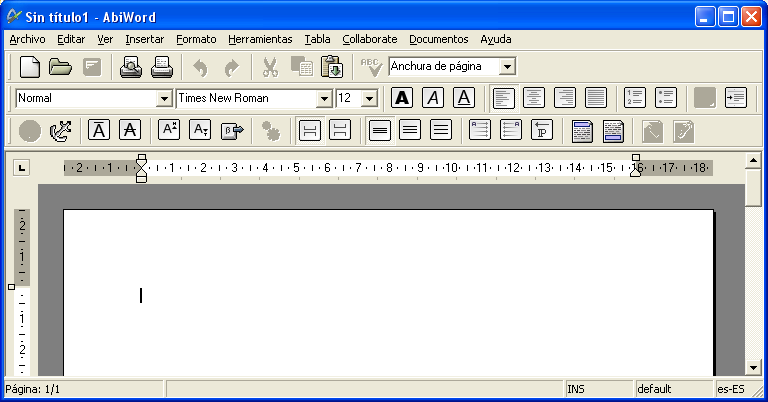
\includegraphics[width=1\textwidth]{abiword_windows.png}
\renewcommand{\figurename}{Fig.}
\caption{Visualización de Abiword en Windows}
\label{contexto:figura}
\end{figure}

Por otro lado en un sistema GNU/Linux se visualiza como:

\begin{figure}[H]
\centering
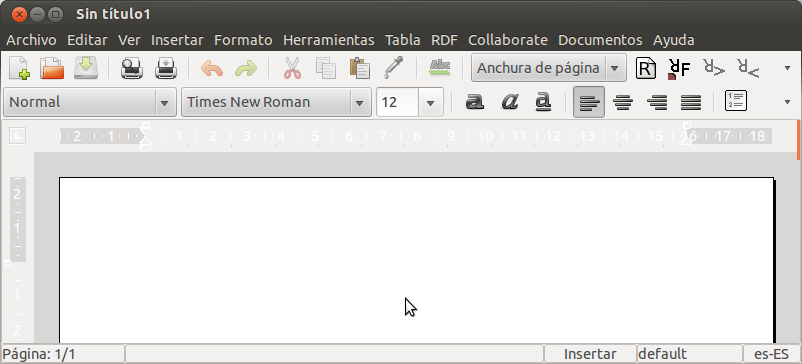
\includegraphics[width=1\textwidth]{abiword_linux.png}
\renewcommand{\figurename}{Fig.}
\caption{Visualización de Abiword en Linux}
\label{contexto:figura}
\end{figure}


Una de las diferencias entre Abiword y la mayoría de los procesadores de texto, es el formato de archivo nativo que utiliza. Abiword utiliza un formato basado en XML, lo cual permite ver el documento con cualquier editor de texto. Así mismo, la aplicación permite trabajar con otros formatos como por ejemplo, DOC, DOCX, ODT, RTF, HTML/XHTML. Para hacer esto, la aplicación utiliza importadores y exportadores. Algunos de estos ya vienen incorporados en la aplicación, mientras que otros son plug-ins\footnote{\url{http://www.abisource.com/wiki/PluginMatrix}}, lo cual permite instalar solo los que uno necesite utilizar, haciendo más liviana la aplicación. 


\subsection{Gnumeric}

Gnumeric es una hoja de cálculo libre que forma parte del entorno de escritorio GNOME. Las características que ofrece lo convierten en un programa versátil y poderoso. 

Gnumeric es un software libre con licencia GPL\footnote{\url{http://www.gnumeric.org/}}. Actualmente la versión disponible para descarga puede ser utilizada únicamente en los sistemas GNU/Linux. Desde Agosto de 2014 no está disponible para sistemas Windows, a raíz de fallos  que se presentan por el uso de Gtk+ que aún no han sido solucionados por no contar con los recursos necesarios.

Al igual que Abiword, tiene bajos requerimientos técnicos pero dota al usuario con una planilla rápida, sencilla y muy completa para usar. La interfaz es muy simple, tal como se puede observar a continuación:

\begin{figure}[H]
\centering
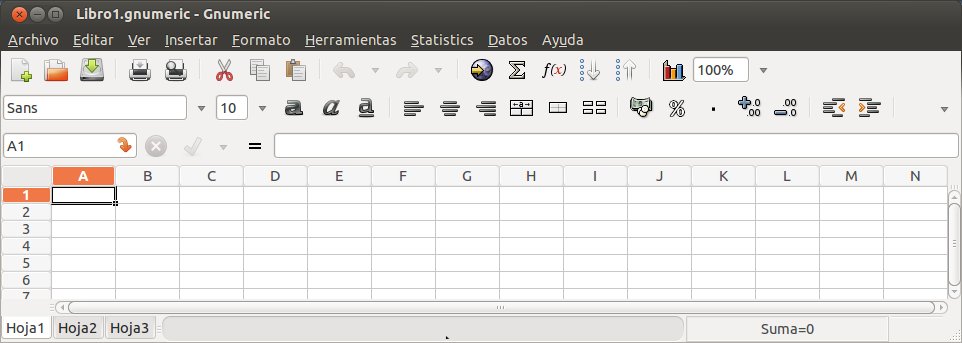
\includegraphics[width=1\textwidth]{gnumeric_linux.png}
\renewcommand{\figurename}{Fig.}
\caption{Visualización de Gnumeric en Linux}
\label{contexto:figura}
\end{figure}

En cuanto al formato de archivo, Gnumeric usa en forma nativa XML comprimido con gzip. Pero la aplicación permite trabajar con otros formatos como por ejemplo, XLS, XLSX, ODS (ODF 1.2), CSV, TXT, HTML\footnote{\url{https://help.gnome.org/users/gnumeric/stable/gnumeric.html\#sect-file-formats}}. Muchos de estos formatos son provistos por medio de plugins. Los plugins en uso se muestran por medio del Plugin Manager de la aplicación\footnote{\url{https://help.gnome.org/users/gnumeric/stable/gnumeric.html\#sect-configuration-plugins}} y desde allí se pueden activar o desactivar todos los que sean necesarios. 

\section{Compatibilidad entre aplicaciones libres y privativas}

Por cuestiones de interoperabilidad, muchas veces es necesario que los archivos que creamos en cualquiera de las aplicaciones libres sean luego manipulados desde aplicaciones propietarias, tales como MS Office, o viceversa. 

En el caso de Microsoft, ya en el 2006 anunció la creación del proyecto ``Open XML Translator''\footnote{\url{http://www.microsoft.com/en-us/news/press/2006/jul06/07-06opensourceprojectpr.aspx}}, para crear una herramienta que sirviera de puente entre el formato Open XML de MS Office y el formato OpenDocument. Además, dicha herramienta sería desarrollada y patentada como software open source. En el 2007, la misma fue finalizada y puesta a disposición bajo el nombre ``OpenXML/ODF Translator Add-ins for Office'' en sourceforge.net con licencia BSD\footnote{\url{http://sourceforge.net/projects/odf-converter/}}, para las aplicaciones Word, Excel y Powerpoint de la suite Microsoft Office 2007, Office 2003 and Office XP. Pero a pesar de esto, habían características que no eran compatibles entre uno y en otro\footnote{\url{http://odf-converter.sourceforge.net/features.html}}. Luego, en el año 2009, con el lanzamiento del Service Pack 2 para la misma suite, entre otras cosas, se agregó a la misma compatibilidad con el formato OpenDocument 1.1 para las aplicaciones ya mencionadas.

Sun Microsystems también creó una herramienta llamada ``ODF plugin for Microsoft Office''\footnote{\url{http://www.oracle.com/us/products/031003.htm}}, el cual permite que MS Office lea y escriba documentos con formato ODF. Este plugin funciona con Microsoft Office 2007 Service Pack 1, Microsoft Office 2003, XP and Microsoft Office 2000, pero ya no está disponible en la página oficial.

Por otro lado, las aplicaciones Word, Excel y Powerpoint de la suite 2010, incluyeron la compatibilidad con ODF 1.1. Para ello, Microsoft agregó una pantalla de selección de formato de archivo que permite al usuario seleccionar el formato de archivo predeterminado para estos productos\footnote{\url{http://office.microsoft.com/es-ar/excel-help/compatibilidad-con-el-formato-opendocument-en-microsoft-office-2010-HA101878944.aspx}}, pudiendo optar entre el formato Office Open XML y el OpenDocument. Este plugin permitía una mejor compatibilidad en el uso del formato ODF por parte de MS Office.

Sin embargo, la compatibilidad no es al 100\%. Ambas suites ofrecen características que no se implementan de la misma manera. Por ello los usuarios de MSOffice que guarden documentos en formato ODF, utilizando características que son parcialmente compatibles o incompatibles, experimentan cambios a la hora de volver a editar el documento y en ocasiones, incluso pérdidas de contenido. Por ello, para cada tipo de aplicación, Microsoft ha publicado información con respecto a la compatibilidad existente:
\begin{itemize}
\item Hoja de cálculo de OpenDocument (.ods) y el formato Excel (.xlsx)\footnote{\url{http://office.microsoft.com/es-ar/excel-help/diferencias-entre-el-formato-hoja-de-calculo-de-opendocument-ods-y-el-formato-excel-xlsx-HA010355787.aspx?CTT=5\&origin=HA101878944}}
\item Presentación de OpenDocument (.odp) y el formato PowerPoint (.pptx)\footnote{\url{http://office.microsoft.com/es-ar/powerpoint-help/diferencias-entre-el-formato-presentacion-de-opendocument-odp-y-el-formato-powerpoint-pptx-HA010355786.aspx?CTT=5\&origin=HA101878944}}
\item Texto de OpenDocument (.odt) y el formato Word 2007 (.docx)\footnote{\url{http://office.microsoft.com/es-ar/word-help/diferencias-entre-el-formato-texto-de-opendocument-odt-y-el-formato-word-2007-docx-HA010355788.aspx?CTT=5\&origin=HA101878944}}
\end{itemize}

Las suites mencionadas anteriormente ofrecen cierto grado de compatibilidad con el formato ODF 1.1. Sin embargo, se presentaron varias críticas\footnote{\url{http://homembit.com/2009/05/microsoft-ahora-intenta-fragmentar-el-odf.html}}\footnote{\url{http://www.robweir.com/blog/2009/05/update-on-odf-spreadsheet-interoperability.html}}. Una de las razones es que desde la versión 3.0, OpenOffice soporta el formato ODF 1.2\footnote{\url{http://www.openoffice.org/marketing/3.0/featurelistbeta.html\#ODF\_1.2\_support}}, mientras que la compatibilidad ofrecida con MS Office es para la versión 1.1. Sin embargo, la suite 2013 de MS Office ya ofrece soporte para ODF 1.2\footnote{\url{http://blogs.office.com/2012/08/13/new-file-format-options-in-the-new-office/}}, aunque de nuevo, esto no asegura compatibilidad al 100\%. Esta es una cuestión muy importante a tener en cuenta cuando se intercambia un archivo para ser usado tanto por aplicaciones libres como privativas. Debemos estar atento a qué versión de ODF se está usando.

En el caso de OpenOffice, es posible cambiar la versión de ODF utilizada para guardar los archivos.

\begin{figure}[H]
\centering
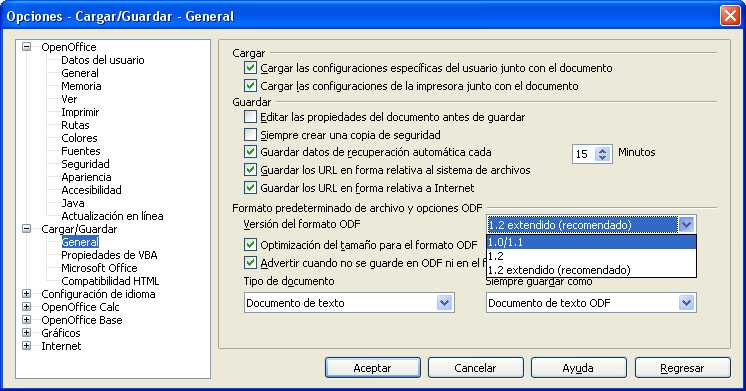
\includegraphics[width=1\textwidth]{cambio_version_odf.png}
\renewcommand{\figurename}{Fig.}
\caption{Elección del tipo de archivo predeterminado}
\label{contexto:figura}
\end{figure}

Entonces, siempre que un archivo con formato ODF deba ser abierto con una versión de MS Office anterior a la 2013, es recomendable elegir en esta configuración, la versión 1.0/1.1. Igualmente se debe tener en cuenta que en lo referido a planillas de cálculo, el formato ODF tuvo varias mejoras en la versión 1.2. Por lo tanto hay que realizar un análisis de compatibilidad antes de decidir con qué versión trabajar por defecto.

En el caso de LibreOffice, también permite realizar este cambio en la configuración por defecto.

\section{Conclusión}

Como pudimos ver, existe un amplio abanico a la hora de seleccionar la aplicación que vamos a utilizar. Una suite que quedó fuera del alcance de este documento es Calligra\footnote{\url{https://www.calligra.org/}}, basada en la plataforma KDE, que también usa el formato OpenDocument y en la que todos los componentes son liberados bajo licencias de software libre. Pero sin importar la suite o aplicación utilizada, siempre es necesario estar atento a la compatibilidad entre las diferentes aplicaciones que se utilizarán. Además, en lo que respecta a ofimática hay mucho movimiento, por lo que es necesario estar actualizado. 

Esto permitirá dar un mejor soporte al usuario que realiza las tareas de ofimática y que el mismo no se desaliente con el uso de las mismas, particularmente en el caso en que esté acostumbrado a utilizar aplicaciones privativas.

\section{Licencia}
Copyright (C) 2014 Claudia Rozas.

Se concede autorización para copiar, distribuir y/o modificar este documento
bajo los términos de la Licencia Creative Commons Atribución-CompartirDerivadasIgual 3.0 Unported. 

http://creativecommons.org/licenses/by-sa/3.0/
\end{document}

